%!TEX root = ../../main.tex
\section{PSU}
I ethvert system er man nødt til at tænke på hvordan de forskellige del-elementer skal forsynes. Der vil blive kigget på den maksimale strøm for hver del. Der forekommer følgende behov for systemet:

\begin{itemize}
\item Pumpen PWM-styres ved 12V. Ved 100\% positiv duty cycle, vil den trække 3A.
\item Ventiler forsynes med 12V. Den vil trække op til 0,5A. Prototypen består maksimalt af 4 ventiler, derfor regnes der med 2A til ventiler.
\item Resten af systemet skal forsynes med 5V. Det består af:	
		\begin{itemize}
		\item Central Control. Består af en Raspberry Pi 2. I databladet står det, at den trækker imellem 600 - 2000mA. 
		\item Flowmåler. Bruger typisk 15mA. Der ser derfor bort fra dette forbrug.
		\item Kar- og Ø-controller. Består af en PSoC som kan forsynes via. USB. Et maksimalt bud vil derfor være 0,5A pr. styk. Prototypen består maksimalt af  4 PSoCs, altså 2A.
		\item RSConverterer. Forbruget er udregnet til ca. 150mA. Prototypen består maksimalt af 5, altså 0,75A.
		\end{itemize}
\end{itemize}

Specifikationerne for 12V- og 5V-forsyningen er nu givet. Disse specifikationer lægges sammen til et samlet system, som vil bestå af følgende udgange:

\begin{itemize}
\item Udgang 1: 5V - 4,75A.
\item Udgang 2: 12V - 5A. 
\end{itemize}

12V- og 5V-forsyningen deles op i 2 kredsløb. Det skyldes at der udnyttes 2 forskellige udtag på en transformer. De kan begge ses herunder.

\begin{figure}[H]
	\centering
	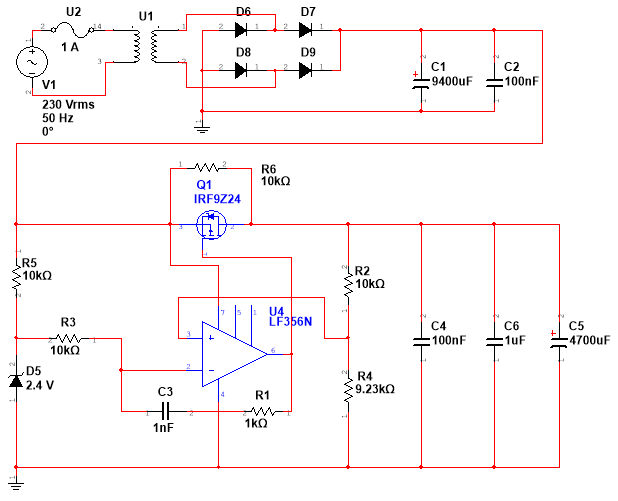
\includegraphics[scale=0.5]{../Hardware/PSU/PSU_5V}
	\caption{Strømforsyning til 5V}
	\label{photo:PSU_5V}
\end{figure}

\begin{figure}[H]
	\centering
	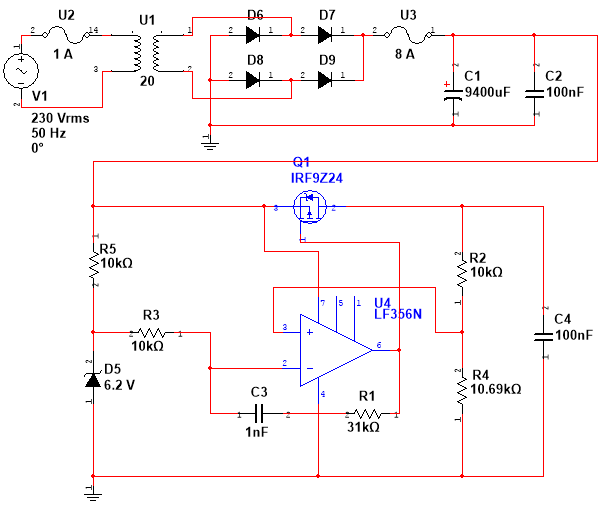
\includegraphics[scale=0.5]{../Hardware/PSU/PSU_12V}
	\caption{Strømforsyning til 12V}
	\label{photo:PSU_12V}
\end{figure}

Der bruges en 230V til 2x12V transformer som maksimalt kan trække 6,6A/udgang. Da kravet til strømforsyningen ligger tæt derpå, vil reguleringskredsløbet også blive opbygget til at kunne håndtere samme strøm som transformatoren.
\\\\
Brokoblingen er af typen 36MB120A. Den er iflg. databladet rated op til 1200V og 35A. Da der kun er tale om 12V og 6,6A, er den mere end kvalificeret.
\\\\
Til at håndtere den skiftende udgangsspænding af brokoblingen, benyttes en 4700uF/25V kondensator. Jo mere kapacitet jo mere stabil vil spændingen være. Det kræver dog også en højere strøm at lade dem op. Det forventes at brokoblingen og transformatoren kan klare dette.
\\\\
Regulerings kredsløbet består af R3, R5, D5, Q1 og Q2. $R_L$ simulerer belastningen. Den eneste komponent som kommer i kontakt med de store strømme, er Q1. Der er her valgt en IRF9Z24, som har følgende ratings:
\\\\
\begin{equation}
	V_{DS} = -60V
\end{equation}
\begin{equation}
	I_D = 11A
\end{equation}
\begin{equation}
	P_D = 60W
\end{equation}
\\\\
Både $V_{DS}$ og $I_D$ er store nok til formålet. Det skal nu beregnes hvorvidt den kan klare den effekt som bliver afsat. Strømmen er ens i de 2 forsyninger. Spændingsfaldet over FET'en vil være størst i 5V-forsyningen. Der regnes med at den uregulerede spænding er 14V.
\\\\
\begin{equation}
	P_D = U * I = (14V - 5V) * 6,6A = 59,4W
\end{equation}
\\\\
Effekten ved maksimal belastning er utrolig tæt på den maksimale rating af FET'en. Det skal dog noteres at den maksimale forventede strøm i 5V-forsyningen er 4,75A, derfor bringer det effekten ned til:
\\\\
\begin{equation}
	P_D = U * I = (14V - 5V) * 4,75A = 42,75W
\end{equation}
\\\\
Dette ligger 25\% under den maksimale rating, hvilket anses for at være acceptabelt. I tilfælde af at 5V-forsyningen skal udnyttes til det fulde, kan der benyttes 2 regulerings kredsløb.

\fxnote{Scopebilleder, forklaringer osv.}